% Options for packages loaded elsewhere
\PassOptionsToPackage{unicode}{hyperref}
\PassOptionsToPackage{hyphens}{url}
%
\documentclass[
  letterpaper,
]{book}

\usepackage{amsmath,amssymb}
\usepackage{iftex}
\ifPDFTeX
  \usepackage[T1]{fontenc}
  \usepackage[utf8]{inputenc}
  \usepackage{textcomp} % provide euro and other symbols
\else % if luatex or xetex
  \usepackage{unicode-math}
  \defaultfontfeatures{Scale=MatchLowercase}
  \defaultfontfeatures[\rmfamily]{Ligatures=TeX,Scale=1}
\fi
\usepackage{lmodern}
\ifPDFTeX\else  
    % xetex/luatex font selection
\fi
% Use upquote if available, for straight quotes in verbatim environments
\IfFileExists{upquote.sty}{\usepackage{upquote}}{}
\IfFileExists{microtype.sty}{% use microtype if available
  \usepackage[]{microtype}
  \UseMicrotypeSet[protrusion]{basicmath} % disable protrusion for tt fonts
}{}
\makeatletter
\@ifundefined{KOMAClassName}{% if non-KOMA class
  \IfFileExists{parskip.sty}{%
    \usepackage{parskip}
  }{% else
    \setlength{\parindent}{0pt}
    \setlength{\parskip}{6pt plus 2pt minus 1pt}}
}{% if KOMA class
  \KOMAoptions{parskip=half}}
\makeatother
\usepackage{xcolor}
\setlength{\emergencystretch}{3em} % prevent overfull lines
\setcounter{secnumdepth}{5}
% Make \paragraph and \subparagraph free-standing
\makeatletter
\ifx\paragraph\undefined\else
  \let\oldparagraph\paragraph
  \renewcommand{\paragraph}{
    \@ifstar
      \xxxParagraphStar
      \xxxParagraphNoStar
  }
  \newcommand{\xxxParagraphStar}[1]{\oldparagraph*{#1}\mbox{}}
  \newcommand{\xxxParagraphNoStar}[1]{\oldparagraph{#1}\mbox{}}
\fi
\ifx\subparagraph\undefined\else
  \let\oldsubparagraph\subparagraph
  \renewcommand{\subparagraph}{
    \@ifstar
      \xxxSubParagraphStar
      \xxxSubParagraphNoStar
  }
  \newcommand{\xxxSubParagraphStar}[1]{\oldsubparagraph*{#1}\mbox{}}
  \newcommand{\xxxSubParagraphNoStar}[1]{\oldsubparagraph{#1}\mbox{}}
\fi
\makeatother


\providecommand{\tightlist}{%
  \setlength{\itemsep}{0pt}\setlength{\parskip}{0pt}}\usepackage{longtable,booktabs,array}
\usepackage{calc} % for calculating minipage widths
% Correct order of tables after \paragraph or \subparagraph
\usepackage{etoolbox}
\makeatletter
\patchcmd\longtable{\par}{\if@noskipsec\mbox{}\fi\par}{}{}
\makeatother
% Allow footnotes in longtable head/foot
\IfFileExists{footnotehyper.sty}{\usepackage{footnotehyper}}{\usepackage{footnote}}
\makesavenoteenv{longtable}
\usepackage{graphicx}
\makeatletter
\def\maxwidth{\ifdim\Gin@nat@width>\linewidth\linewidth\else\Gin@nat@width\fi}
\def\maxheight{\ifdim\Gin@nat@height>\textheight\textheight\else\Gin@nat@height\fi}
\makeatother
% Scale images if necessary, so that they will not overflow the page
% margins by default, and it is still possible to overwrite the defaults
% using explicit options in \includegraphics[width, height, ...]{}
\setkeys{Gin}{width=\maxwidth,height=\maxheight,keepaspectratio}
% Set default figure placement to htbp
\makeatletter
\def\fps@figure{htbp}
\makeatother

\makeatletter
\@ifpackageloaded{bookmark}{}{\usepackage{bookmark}}
\makeatother
\makeatletter
\@ifpackageloaded{caption}{}{\usepackage{caption}}
\AtBeginDocument{%
\ifdefined\contentsname
  \renewcommand*\contentsname{Table of contents}
\else
  \newcommand\contentsname{Table of contents}
\fi
\ifdefined\listfigurename
  \renewcommand*\listfigurename{List of Figures}
\else
  \newcommand\listfigurename{List of Figures}
\fi
\ifdefined\listtablename
  \renewcommand*\listtablename{List of Tables}
\else
  \newcommand\listtablename{List of Tables}
\fi
\ifdefined\figurename
  \renewcommand*\figurename{Figure}
\else
  \newcommand\figurename{Figure}
\fi
\ifdefined\tablename
  \renewcommand*\tablename{Table}
\else
  \newcommand\tablename{Table}
\fi
}
\@ifpackageloaded{float}{}{\usepackage{float}}
\floatstyle{ruled}
\@ifundefined{c@chapter}{\newfloat{codelisting}{h}{lop}}{\newfloat{codelisting}{h}{lop}[chapter]}
\floatname{codelisting}{Listing}
\newcommand*\listoflistings{\listof{codelisting}{List of Listings}}
\makeatother
\makeatletter
\makeatother
\makeatletter
\@ifpackageloaded{caption}{}{\usepackage{caption}}
\@ifpackageloaded{subcaption}{}{\usepackage{subcaption}}
\makeatother

\ifLuaTeX
  \usepackage{selnolig}  % disable illegal ligatures
\fi
\usepackage{bookmark}

\IfFileExists{xurl.sty}{\usepackage{xurl}}{} % add URL line breaks if available
\urlstyle{same} % disable monospaced font for URLs
\hypersetup{
  pdftitle={Weikersheim, Residenzschloss},
  pdfauthor={Team Redaktion},
  hidelinks,
  pdfcreator={LaTeX via pandoc}}


\title{Weikersheim, Residenzschloss}
\author{Team Redaktion}
\date{2024-03-22}

\begin{document}
\frontmatter
\maketitle

\renewcommand*\contentsname{Table of contents}
{
\setcounter{tocdepth}{2}
\tableofcontents
}

\mainmatter
\bookmarksetup{startatroot}

\chapter{Katalog zur Ausstellung: Der Große Saal
(Rittersaal)}\label{katalog-zur-ausstellung-der-grouxdfe-saal-rittersaal}

Ein Katalog mit Kunstwerken aus der CbDD-Sammlung. Textteil:
\href{https://www.deckenmalerei.eu/42d06165-58e7-4653-bfe4-3d5f7091fc33\#6e73f774-4b7f-4e37-937b-e11cc35c5bc8}{6e73f774-4b7f-4e37-937b-e11cc35c5bc8}

Großer Saal (Rittersaal) {[}Raum{]} Name: Großer Saal (Rittersaal) ID:
15685f4a-3727-4110-8967-1d8287431997 Typ: Raum Länge (m): 36.4 Breite
(m): 11.7 Höhe (m): 8.25 Funktion {[}Raum{]}: Saal -\textgreater{}
Hauptsaal Datierung {[}Raum{]}: 1601-1605 hat Auftraggeber: Wolfgang
II., Hohenlohe-Weikersheim, Graf {[}Person{]} hat Auftraggeber: Carl
Ludwig, Hohenlohe-Weikersheim, Graf {[}Person{]} hat Teil: Malerei des
Barock {[}Malerei{]} hat Teil: Malerei der Renaissance {[}Malerei{]} hat
Stuckateur: Schmidt, Gerhard {[}Person{]} hat Stuckateur: Limmerich,
Christoph {[}Person{]} hat Bildhauer: Juncker, Michael {[}Person{]} ist
dokumentiert in: Der Große Saal (Rittersaal) {[}Textteil{]} ist Teil
von: Erschließungsraumfolgen {[}Raumfolge{]} Erstellung des Datensatzes:
2020-05-19, 11:18 letzte Bearbeitung: 2023-10-16, 14:28

This work is licensed under a Creative Commons
Attribution-NonCommercial-NoDerivs 4.0 International License.

\bookmarksetup{startatroot}

\chapter{Impressum}\label{impressum}

Veröffentlichungsmetadaten, die aus dem Thoth.pub GraphQL API.
\url{https://api.thoth.pub/graphiql}

Katalog zur Ausstellung: Der Große Saal (Rittersaal) Weikersheim,
Residenzschloss

Open Science Lab - TIB Hannover

First published 2024-04-16

Copyright © The authors 2024 Licensed as
https://creativecommons.org/licenses/by-nc-nd/4.0/

DOI: https://doi.org/10.5281/zenodo.10977822

\bookmarksetup{startatroot}

\chapter{Essay}\label{essay}

Get data of text items from wikibase

Wikibase link:
\url{https://computational-publishing-service.wikibase.cloud/entity/Q209}

Kurator: Seeger, Ulrike

Bau-, Ausstattungs- und Funktionsgeschichte

Die hervorragend erhaltene wandfeste Ausstattung des Großen Saals, der
1639 als „großer Saahl`` {[}1{]} geführt wurde und seinen heute
geläufigen Namen Rittersaal erst im Nachhinein erhielt, datiert aus den
Jahren 1601 bis 1605. Am Beginn stand den Quellen zufolge der
monumentale Saalkamin. Der Vertrag mit dem Bildhauer Michael Juncker aus
Miltenberg datiert vom 7. September 1601.{[}2{]} Im November 1601 wurden
mit Balthasar Katzenberger die Deckengemälde verdingt, der die Arbeiten
13 Monate später Anno 1602 abschloss.{[}3{]} 1603 signierte und datierte
der Kalkschneider Gerhard Schmidt das Portal an der inneren
Ostseite.{[}4{]} Die Jahreszahl 1605 zusammen mit den Initialen CL für
den Kalkschneider Christoph Limmerich über der Tür zum Altan markieren
den Abschluss der Arbeiten.{[}5{]}

Seit 1710/11 wurde der Saal unter Graf Carl Ludwig behutsam dem barocken
Zeitgeschmack angepasst und inhaltlich vom Jagd- zum gräflichen
Rittersaal umgedeutet. Christian Thalwitzer hatte Balthasar
Katzenbergers Deckengemälde „im großen Saal {[}zu{]} übermahlen, genau
durch{[}zu{]}gehen und wo es Schaden genommen, mit allem Fleyß``
auszubessern.{[}6{]} Bei dieser Gelegenheit versah er die Gemälderahmen
und die dazwischenliegenden Stuckrippen mit der bis heute gültigen roten
Marmorierung.{[}7{]} An den Wänden wurden die Roll- und
Beschlagwerkkartuschen der Schmuckzone ebenfalls rot marmoriert und an
Kamin und Innenportal die rot marmorierten Schattenrahmen hinzugefügt.

In einem zweiten Schritt wurde der Sockel ringsum mit rot marmorierten
Lambris versehen, die Christian Thalwitzer im Rechnungsjahr 1715/16 mit
51 Schloss- und Gartenveduten im Querformat{[}8{]} und 27 Orangenbäumen
und anderen exotischen Kübelpflanzen im Hochformat bemalte. Die 12
ganzfigurigen Porträts männlicher Vorfahren zum Teil in Ritterrüstung,
die dem Rittersaal seinen heutigen Namen gaben, schuf bereits 1710 Peter
Franz Tassaert aus Rothenburg.{[}9{]}

Beschreibung des Raumes

Der 36,4 Meter lange, 11,7 Meter breite und 8,25 Meter hohe Saal{[}10{]}
wird durch hohe segmentbogenförmige Fensternischen gegliedert, deren
Achsen von großen Okuli weitergeführt werden. Im Gegenzug zu dieser
Vertikalen beschränkt sich der reiche Stuckdekor friesartig auf die
obere Wandzone, die oberhalb eines Gesimses auf der Höhe des oberen
Drittels der Fenster beginnt. Dadurch, dass sich die Stuckdekoration in
das obere Drittel der Fensterlaibungen hineinzieht, erwecken sie den
Eindruck hoheitsvoll gestelzter Bögen.{[}11{]}

An der Westwand, neben der im ersten Joch der Hofseite der Saal über die
Wendeltreppe betreten wird, erhebt sich ein monumentaler Kamin. Mit
Kaminöffnung, Attikafeld und rundbogigem Auszug umfasst er drei Zonen,
von denen Attika und Auszug in der Höhe der stuckierten Wandzone des
Saals entsprechen. An der Ostwand, wo man den Saal Richtung Tafelstube
verlässt, befindet sich ein prächtiges, 1603 datiertes stuckiertes
Innenportal des Kalkschneiders Gerhard Schmidt.{[}12{]} Darüber
verläuft, teilweise hinter dem Attikarelief, eine Empore beispielsweise
für Musiker.

Den Kamin flankieren stuckierte Darstellungen des Grafenpaars Wolfgang
II. von Hohenlohe und Magdalena, geborene Prinzessin von
Nassau-Katzenelnbogen mit ihrer jeweiligen Ahnenprobe.{[}13{]} Dem Graf
wurde die zeremoniell höherrangige Seite heraldisch rechts des Kamins,
der Gräfin die Seite heraldisch links des Kamins zugeteilt. Graf und
Gräfin liegen jeweils auf der Seite einander abgewandt und blicken mit
aufgestütztem Kopf in den Saal. Aus ihnen heraus wächst in der Art einer
Wurzel Jesse die über fünf Generationen geführte Ahnenprobe. Der Graf
trägt eine Rüstung mit Waffenrock und stützt seinen Ellenbogen auf einen
Helm. Die Gräfin hat zwei Kinder im Arm, von denen das vordere ein Junge
ist.

An den beiden Längsseiten nimmt die stuckierte Schmuckzone weit
vorkragende, gleichfalls stuckierte Wandskulpturen wilder Tiere auf. Sie
beziehen sich einerseits auf das Programm der Decke, das der höfischen
Jagd in all ihren Ausformungen gewidmet ist. Andererseits sind sie auf
die Kaminwand ausgerichtet, die mit ihren nachstehend zu erläuternden
Bildthemen als Stellvertreter des Grafen, seiner konfessionellen
Einstellung und seiner dynastischen Herkunft konzipiert ist. Zusammen
mit einer gemalten Darstellung des lyraspielenden Orpheus an der Decke
erlauben die Tiere in ihrer Ausrichtung auf den Kamin die Identifikation
des Grafen mit Orpheus als Sinnbild des guten Herrschers. Diese hier
erstmals entwickelte Deutung wird unten im Abschnitt „Programm und
Synthese der Saalausstattung der Renaissance`` vorgetagen.

Kamin und Innenportal

Der Kamin aus Andernacher Tuffstein von Michael Juncker und seinen
Söhnen Hans und Zacharias aus Miltenberg präsentiert im Hauptrelief als
zentrales Motiv die persönliche Devise des Grafen Wolfgang. Die
Entschlüsselung der im Vertrag vom September 1601 vereinbarten „ihrer
gnaden Diviso``{[}14{]} gelang erst vor wenigen Jahren Jürgen
Kniep.{[}15{]} Dargestellt ist ein antikisch gekleideter Krieger,
umgeben von den Symbolen der Kardinal- und theologischen Tugenden. Die
Devise „Gott gibt Glück`` lässt den reformatorischen Glauben des Grafen
Wolfgang ebenso erkennen wie die Betonung der Liebe (Herz in der linken
Hand des Kriegers) und des Buches, aus dem die Schlange ihre Weisheit
bezieht. Im Sinne der protestantischen Rechtfertigungslehre oblag es
nicht dem Klerus, sondern allein Gott, dem Menschen Gnade angedeihen zu
lassen.

Als räumliches Gegenstück zum skulptierten Kamin entstand 1603 in einem
Paragone der Techniken und Materialien das monumentale, aus Stuck
gefertigte Innenportal an der Ostseite. Sein Aufbau ist wie der Kamin
dreizonig mit rundbogiger Öffnung, Attikarelief und Auszug. Der
Kalkschneider Gerhard Schmidt, der das Portal selbstbewusst mit seinen
Initialen signiert hat, hat in der Türkenschlacht des Hauptreliefs mit
extrem hinterschnittenen Pferde- und Soldatenleibern den moderater
skulptierten Steinkamin an Kunstfertigkeit übertroffen. Einen Höhepunkt
der Stuckateurskunst der Zeit bildet der vollplastisch gearbeitete
heilige Georg auf seinem zum Sprung über den Drachen ansetzenden Pferd.

Das Portal ist inhaltlich auf den ältesten Sohn des Grafen Wolfgang,
Georg Friedrich, zu beziehen, der im Rang eines Obristen des Fränkischen
Reichskreises und auch der kaiserlichen Armee im Langen Türkenkrieg
(1593--1606) kämpfte.{[}16{]} Als einer seiner größten Erfolge gilt die
versuchte Einnahme der Festung Gran (Eszergom) im Jahr 1594, an der er
als kaiserlicher Obrist beteiligt war.{[}17{]} Die Festung, vor der sich
auf dem Relief das Schlachtengetümmel abspielt, stellt in der Tat
Eszergom da, was an der Höhenlage und der Zweiturmfassade der Kathedrale
zu erkennen ist.{[}18{]} Der das Portal bekrönende heilige Georg als
Drachentöter mit Lanze und zugleich Namenspatron des Erbprinzen sowie
Patron der Stadtkirche wäre im Sinne des Protestantismus als
tugendhafter Bezwinger des Bösen zu deuten.{[}19{]} Mit der Thematik des
Langen Türkenkriegs bereitete das Portal auf die dahinterliegende
Tafelstube vor, für deren Decke Balthasar Katzenberger 12 große
Belagerungsszenen auf Leinwand malte.

Das Portal von 1603 war aber nicht nur heroisch gestimmt. In den
Zwickeln lagern Putti, die als Mahnung an die Endlichkeit des Lebens dem
Betrachter ein Stundenglas, eine Sense und einen Schlüssel -- vielleicht
ins Himmelreich -- vor Augen halten.

Das Mobiliar

Die renaissancezeitliche Ausstattung des Saals mit Mobilien geht aus
einem 1625--1627 aufgenommenen Inventar hervor.{[}20{]} Die als erstes
genannten „Ein und zwanzig Stuck goldt uf Leder tappezerey`` dürften als
goldgeprägte Ledertapeten die Trumeaus zwischen den Fenstern geziert
haben. Ledertapeten waren kostbar, was sich in ihrer erstplatzierten
Nennung niederschlug.{[}21{]} An Stellmöbeln beinhaltete der Saal „Zwo
lange Tafel`` und „Ein und dreissig von goldt uff Lederne Sessel``. Die
Wände schmückten zusätzlich zu den Ledertapeten „Sechzehn gemahlte
Tafeln``, also im Sujet nicht näher charakterisierte Gemälde. Die
Beleuchtung erfolgte über „Acht große hülzerne Lichter, gemahlt``.

Vier Gemälde wurden zusätzlich zu den sechzehn aufgeführt, da sie
vermutlich im Vorgängerinventar des Grafen Wolfgang, das dem Inventar
als Vorlage diente, noch nicht enthalten waren. Sie stellten „Kaiser
Matthie und der Kayserin / Item Meines Gnd. Herrn und gnl. Frawen
Abcontrafehung`` dar. Kaiser Matthias regierte in den Jahren 1612--1619,
seine Gemahlin Anna von Österreich-Tirol starb 1618. Die Gemälde
stammten demnach aus der Zeit des Grafen Georg Friedrich von
Hohenlohe-Weikersheim, der mit Eva von Waldstein verheiratet war.

{[}1{]} HZAN La 130 Bü 152, Schadensinventar von 1639. Die Kenntnis und
die Transkription dieser Archivalie verdankt die Autorin Frieder
Leipold.

{[}2{]} Der erhaltene Vertrag (HZAN We 50 D6) in Transkription bei
Freeden, Kamin, 1950, S. 144--145. Bezahlt wurde Juncker im Oktober
1602.

{[}3{]} Poser, Deckenbilder, 1980, S. 160--161.

{[}4{]} Merten, Weikersheim, o. J., S. 44. Drös, Inschriften
Mergentheim, 2002, S. 244. Zum Oeuvre und Lebensweg des Kalkschneiders
Gerhard Schmidt: Kreder, Hellenstein, 2005/2006; Rinn-Kupka, Stuck,
2018, S. 126--129; Lange, ‚welsche Kamin`, 2019.

{[}5{]} Merten, Weikersheim, o. J., S. 44. Drös, Inschriften
Mergentheim, 2002, S. 254.

{[}6{]} Fandrey, Weikersheim, 2010, S. 55.

{[}7{]} Dieser Befund kam bei der Restaurierung der Jahre 1995--1997
zutage. Für zahlreiche Informationen und die Übermittlung des
Abschlussberichts vom 05.03.1998 dankt die Autorin Herrn Dipl.-Ing. Erik
Reinhold, Staatliches Hochbauamt Heilbronn.

{[}8{]} Die Vedute des Carlsberg bei Weikersheim kam erst 1747 im
Zusammenhang mit der damals aufgestellten Kunstuhr hinzu, doch dürfte
sie eine ältere Vedute am Fensterpfeiler hinter der Uhr ersetzt haben.

{[}9{]} Valentin, Malerische Lebensläufe, 2019, Anm. 11. Zu Tassaert
liegt ein Lebenslauf mit Werkverzeichnis vor: Schnurrer, Tassaert, 2014.

{[}10{]} Die genauen Maße gibt Walther-Gerd Fleck (Weyer, Georg Stegle,
2017, S. 52).

{[}11{]} Vgl. dagegen Gebeßler, Saal Süddeutschland, 1957, S. 49, der
die Fensternischen aufgrund ihrer Dekoration als Anräume empfindet.

{[}12{]} Das Portal wird in der Literatur zu Unrecht als Eingangsportal
in den Saal beschrieben (Poser, Deckenbilder, 1980, S. 160; Kniep,
Glück, 2005, S. 52 und 59; Käpplinger, Jagd, 2011, S. 73). Es ist jedoch
nach innen gerichtet, führt also von innen nach außen. Außerdem folgt in
der Wegeführung eines Renaissanceschlosses die Tafelstube auf den
Rittersaal. Auch der Betrachterstandpunkt der Deckengemälde ist mit dem
Rücken zum Kamin so ausgerichtet, dass man die Bilder vom Kamin kommend,
Richtung Tafelstube gehend bewundert.

{[}13{]} Zu den Ahnenproben: Drös, Inschriften Mergentheim, 2002, S.
255--261. Außerdem Kniep, Glück, 2005, S. 48--52.

{[}14{]} Freeden, Kamin, 1950, S. 144.

{[}15{]} Kniep, Glück, 2005, S. 57--74. Weiterführende Gedanken und
Literatur zur Bildhauerfamilie Juncker liefert: Lange, ‚welsche Kamin`,
2019.

{[}16{]} Kniep, Glück, 2005, S. 52--57. Außerdem Findbuch HZAN La 130 Bü
102 (Bestallung zum Obristen des Fränkischen Reichskreises, 1598) und La
130 Bü 108 (Teilnahme als kaiserlicher Obrist am Feldzug gegen die
Türken 1603).

{[}17{]} Trentin-Meyer, Georg Friedrich von Hohenlohe, 2019, S. 90. Vgl.
Niederkorn, Langer Türkenkrieg, 1993, S. 11.

{[}18{]} Außerdem als Beleg die Darstellung in: Ortelius, Chronologia,
1602, Tf. „Wahre Contrafactur der Belagerung Gran, sampt der Schlacht so
dabei geschehen, den 3. Augusti. Anno 1595``. Ortelius wählte für seine
Illustration die erfolgreiche Belagerung und Schlacht von 1595. Die
Belagerung von 1594 war für die Kaiserlichen noch nicht erfolgreich.

{[}19{]} Kniep, Glück, 2005, S. 56.

{[}20{]} Auszüge des Inventars stellte freundlicherweise Dinah
Rottschäfer der Autorin zur Verfügung.

{[}21{]} Bei dem von Käpplinger, Auf's Schönste, 2019, S. 189 mit Anm. 3
genannten Inventar von 1634 handelt es sich um einen Schadensbericht, in
dem die Ledertapeten verkürzt als „tappezereien von gold`` bezeichnet
wurden, was Käpplinger in Unkenntnis des Vorgängerinventars als textile
Wandbespannungen deutete.

\bookmarksetup{startatroot}

\chapter{Paintings}\label{paintings}

Get data of image items from wikibase

Wikibase link:
\url{https://computational-publishing-service.wikibase.cloud/entity/Q212}

Title: Rittersaal \& Raum 72 -- nach Westen

Year: 2018

Description: Teil von: Schloss Weikersheim SaalbauWolfgang Beringer,
Baumeister \& Steinmetz - Georg Stegle, Baumeister - Entwurf: Georges
Robin, Architekt - Elias Gunzenhäuser, Zimmermann - Weikersheim,
Marktplatz 11 - ab 1595

\includegraphics{paintings_files/figure-pdf/cell-3-output-2.png}

Wikibase link:
\url{https://computational-publishing-service.wikibase.cloud/entity/Q213}

Title: Löwenpaar -- Gesamtansicht

Year: 2018

Description: Gerhardt Schmidt, Bildhauer - Mitarbeit: Christoph
Limmerich, Bildhauer - Mitarbeit: Caspar Dieterich, Fassmaler -
Weikersheim, Schloss Weikersheim, Rittersaal \& Raum 72 - Vollendung:
1605 - 1747

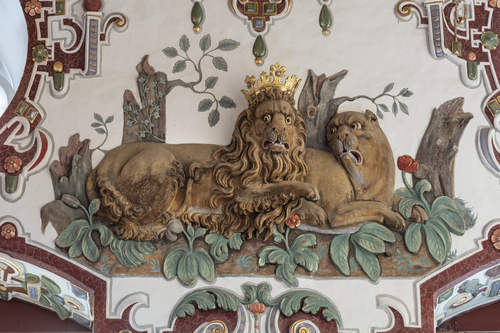
\includegraphics{paintings_files/figure-pdf/cell-3-output-4.png}

Wikibase link:
\url{https://computational-publishing-service.wikibase.cloud/entity/Q214}

Title: Bär -- Gesamtansicht

Year: 2018

Description: Gerhardt Schmidt, Bildhauer - Mitarbeit: Christoph
Limmerich, Bildhauer - Mitarbeit: Caspar Dieterich, Fassmaler -
Weikersheim, Schloss Weikersheim, Rittersaal \& Raum 72 - Vollendung:
1605 - 1747

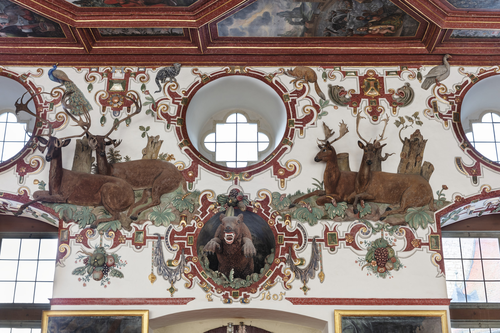
\includegraphics{paintings_files/figure-pdf/cell-3-output-6.png}

Wikibase link:
\url{https://computational-publishing-service.wikibase.cloud/entity/Q215}

Title: Hirschpaare -- Gesamtansicht

Year: 2018

Description: Gerhardt Schmidt, Bildhauer - Mitarbeit: Christoph
Limmerich, Bildhauer - Mitarbeit: Caspar Dieterich, Fassmaler -
Weikersheim, Schloss Weikersheim, Rittersaal \& Raum 72 - Vollendung:
1605 - 1747

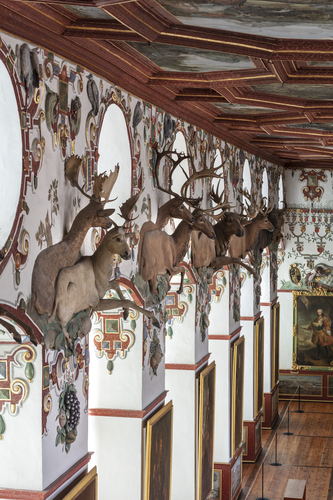
\includegraphics{paintings_files/figure-pdf/cell-3-output-8.png}

Wikibase link:
\url{https://computational-publishing-service.wikibase.cloud/entity/Q216}

Title: Affe -- Gesamtansicht

Year: 2018

Description: Gerhardt Schmidt, Bildhauer - Mitarbeit: Christoph
Limmerich, Bildhauer - Mitarbeit: Caspar Dieterich, Fassmaler -
Weikersheim, Schloss Weikersheim, Rittersaal \& Raum 72 - Vollendung:
1605 - 1747

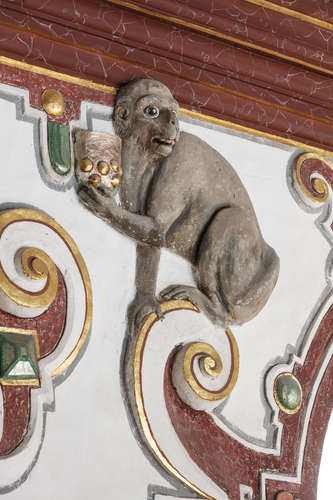
\includegraphics{paintings_files/figure-pdf/cell-3-output-10.png}

Wikibase link:
\url{https://computational-publishing-service.wikibase.cloud/entity/Q200}

Title: Rittersaal \& Raum 72 -- nach Osten

Year: 2018-01-01T00:00:00Z

Description: Teil von: Schloss Weikersheim Saalbau Wolfgang Beringer,
Baumeister \& Steinmetz - Georg Stegle, Baumeister - Entwurf: Georges
Robin, Architekt - Elias Gunzenhäuser, Zimmermann - Weikersheim,
Marktplatz 11 - ab 1595

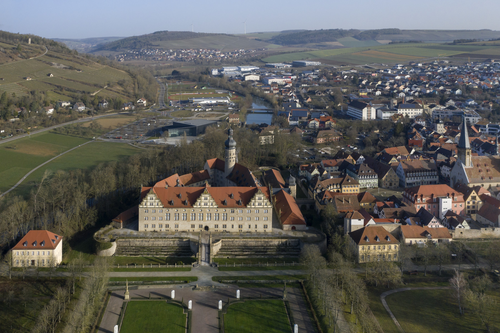
\includegraphics{paintings_files/figure-pdf/cell-3-output-12.png}

Wikibase link:
\url{https://computational-publishing-service.wikibase.cloud/entity/Q211}

Title: Rittersaal \& Raum 72 -- nach Osten

Year: 2018-01-01T00:00:00Z

Description: Teil von: Schloss Weikersheim SaalbauWolfgang Beringer,
Baumeister \& Steinmetz - Georg Stegle, Baumeister - Entwurf: Georges
Robin, Architekt - Elias Gunzenhäuser, Zimmermann - Weikersheim,
Marktplatz 11 - ab 1595

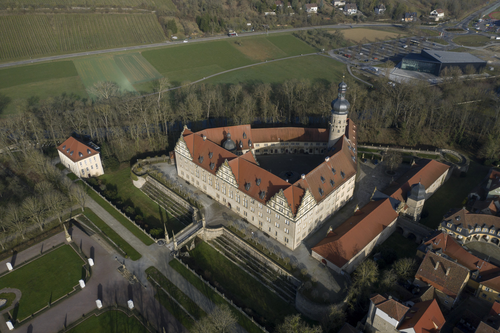
\includegraphics{paintings_files/figure-pdf/cell-3-output-14.png}

Wikibase link:
\url{https://computational-publishing-service.wikibase.cloud/entity/Q212}

Title: Rittersaal \& Raum 72 -- nach Westen

Year: 2018-01-01T00:00:00Z

Description: Teil von: Schloss Weikersheim SaalbauWolfgang Beringer,
Baumeister \& Steinmetz - Georg Stegle, Baumeister - Entwurf: Georges
Robin, Architekt - Elias Gunzenhäuser, Zimmermann - Weikersheim,
Marktplatz 11 - ab 1595

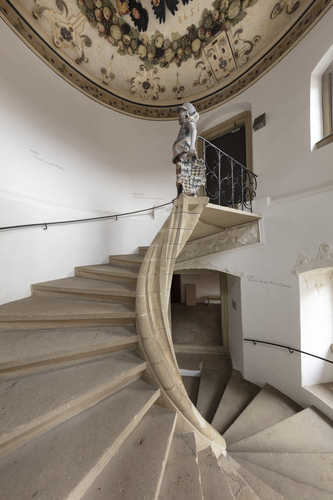
\includegraphics{paintings_files/figure-pdf/cell-3-output-16.png}

Wikibase link:
\url{https://computational-publishing-service.wikibase.cloud/entity/Q213}

Title: Löwenpaar -- Gesamtansicht

Year: 2018-01-01T00:00:00Z

Description: Gerhardt Schmidt, Bildhauer - Mitarbeit: Christoph
Limmerich, Bildhauer - Mitarbeit: Caspar Dieterich, Fassmaler -
Weikersheim, Schloss Weikersheim, Rittersaal \& Raum 72 - Vollendung:
1605 - 1747

\begin{verbatim}
ConnectTimeout: HTTPSConnectionPool(host='previous.bildindex.de', port=443): Max retries exceeded with url: /bilder/fmd10005864a.jpg (Caused by ConnectTimeoutError(<urllib3.connection.HTTPSConnection object at 0x0000010A5ECAE750>, 'Connection to previous.bildindex.de timed out. (connect timeout=None)'))
---------------------------------------------------------------------------
TimeoutError                              Traceback (most recent call last)
File ~\AppData\Local\Packages\PythonSoftwareFoundation.Python.3.11_qbz5n2kfra8p0\LocalCache\local-packages\Python311\site-packages\urllib3\connection.py:203, in HTTPConnection._new_conn(self)
    202 try:
--> 203     sock = connection.create_connection(
    204         (self._dns_host, self.port),
    205         self.timeout,
    206         source_address=self.source_address,
    207         socket_options=self.socket_options,
    208     )
    209 except socket.gaierror as e:

File ~\AppData\Local\Packages\PythonSoftwareFoundation.Python.3.11_qbz5n2kfra8p0\LocalCache\local-packages\Python311\site-packages\urllib3\util\connection.py:85, in create_connection(address, timeout, source_address, socket_options)
     84 try:
---> 85     raise err
     86 finally:
     87     # Break explicitly a reference cycle

File ~\AppData\Local\Packages\PythonSoftwareFoundation.Python.3.11_qbz5n2kfra8p0\LocalCache\local-packages\Python311\site-packages\urllib3\util\connection.py:73, in create_connection(address, timeout, source_address, socket_options)
     72     sock.bind(source_address)
---> 73 sock.connect(sa)
     74 # Break explicitly a reference cycle

TimeoutError: [WinError 10060] A connection attempt failed because the connected party did not properly respond after a period of time, or established connection failed because connected host has failed to respond

The above exception was the direct cause of the following exception:

ConnectTimeoutError                       Traceback (most recent call last)
File ~\AppData\Local\Packages\PythonSoftwareFoundation.Python.3.11_qbz5n2kfra8p0\LocalCache\local-packages\Python311\site-packages\urllib3\connectionpool.py:790, in HTTPConnectionPool.urlopen(self, method, url, body, headers, retries, redirect, assert_same_host, timeout, pool_timeout, release_conn, chunked, body_pos, preload_content, decode_content, **response_kw)
    789 # Make the request on the HTTPConnection object
--> 790 response = self._make_request(
    791     conn,
    792     method,
    793     url,
    794     timeout=timeout_obj,
    795     body=body,
    796     headers=headers,
    797     chunked=chunked,
    798     retries=retries,
    799     response_conn=response_conn,
    800     preload_content=preload_content,
    801     decode_content=decode_content,
    802     **response_kw,
    803 )
    805 # Everything went great!

File ~\AppData\Local\Packages\PythonSoftwareFoundation.Python.3.11_qbz5n2kfra8p0\LocalCache\local-packages\Python311\site-packages\urllib3\connectionpool.py:491, in HTTPConnectionPool._make_request(self, conn, method, url, body, headers, retries, timeout, chunked, response_conn, preload_content, decode_content, enforce_content_length)
    490         new_e = _wrap_proxy_error(new_e, conn.proxy.scheme)
--> 491     raise new_e
    493 # conn.request() calls http.client.*.request, not the method in
    494 # urllib3.request. It also calls makefile (recv) on the socket.

File ~\AppData\Local\Packages\PythonSoftwareFoundation.Python.3.11_qbz5n2kfra8p0\LocalCache\local-packages\Python311\site-packages\urllib3\connectionpool.py:467, in HTTPConnectionPool._make_request(self, conn, method, url, body, headers, retries, timeout, chunked, response_conn, preload_content, decode_content, enforce_content_length)
    466 try:
--> 467     self._validate_conn(conn)
    468 except (SocketTimeout, BaseSSLError) as e:

File ~\AppData\Local\Packages\PythonSoftwareFoundation.Python.3.11_qbz5n2kfra8p0\LocalCache\local-packages\Python311\site-packages\urllib3\connectionpool.py:1092, in HTTPSConnectionPool._validate_conn(self, conn)
   1091 if conn.is_closed:
-> 1092     conn.connect()
   1094 if not conn.is_verified:

File ~\AppData\Local\Packages\PythonSoftwareFoundation.Python.3.11_qbz5n2kfra8p0\LocalCache\local-packages\Python311\site-packages\urllib3\connection.py:611, in HTTPSConnection.connect(self)
    610 sock: socket.socket | ssl.SSLSocket
--> 611 self.sock = sock = self._new_conn()
    612 server_hostname: str = self.host

File ~\AppData\Local\Packages\PythonSoftwareFoundation.Python.3.11_qbz5n2kfra8p0\LocalCache\local-packages\Python311\site-packages\urllib3\connection.py:212, in HTTPConnection._new_conn(self)
    211 except SocketTimeout as e:
--> 212     raise ConnectTimeoutError(
    213         self,
    214         f"Connection to {self.host} timed out. (connect timeout={self.timeout})",
    215     ) from e
    217 except OSError as e:

ConnectTimeoutError: (<urllib3.connection.HTTPSConnection object at 0x0000010A5ECAE750>, 'Connection to previous.bildindex.de timed out. (connect timeout=None)')

The above exception was the direct cause of the following exception:

MaxRetryError                             Traceback (most recent call last)
File ~\AppData\Local\Packages\PythonSoftwareFoundation.Python.3.11_qbz5n2kfra8p0\LocalCache\local-packages\Python311\site-packages\requests\adapters.py:486, in HTTPAdapter.send(self, request, stream, timeout, verify, cert, proxies)
    485 try:
--> 486     resp = conn.urlopen(
    487         method=request.method,
    488         url=url,
    489         body=request.body,
    490         headers=request.headers,
    491         redirect=False,
    492         assert_same_host=False,
    493         preload_content=False,
    494         decode_content=False,
    495         retries=self.max_retries,
    496         timeout=timeout,
    497         chunked=chunked,
    498     )
    500 except (ProtocolError, OSError) as err:

File ~\AppData\Local\Packages\PythonSoftwareFoundation.Python.3.11_qbz5n2kfra8p0\LocalCache\local-packages\Python311\site-packages\urllib3\connectionpool.py:844, in HTTPConnectionPool.urlopen(self, method, url, body, headers, retries, redirect, assert_same_host, timeout, pool_timeout, release_conn, chunked, body_pos, preload_content, decode_content, **response_kw)
    842     new_e = ProtocolError("Connection aborted.", new_e)
--> 844 retries = retries.increment(
    845     method, url, error=new_e, _pool=self, _stacktrace=sys.exc_info()[2]
    846 )
    847 retries.sleep()

File ~\AppData\Local\Packages\PythonSoftwareFoundation.Python.3.11_qbz5n2kfra8p0\LocalCache\local-packages\Python311\site-packages\urllib3\util\retry.py:515, in Retry.increment(self, method, url, response, error, _pool, _stacktrace)
    514     reason = error or ResponseError(cause)
--> 515     raise MaxRetryError(_pool, url, reason) from reason  # type: ignore[arg-type]
    517 log.debug("Incremented Retry for (url='%s'): %r", url, new_retry)

MaxRetryError: HTTPSConnectionPool(host='previous.bildindex.de', port=443): Max retries exceeded with url: /bilder/fmd10005864a.jpg (Caused by ConnectTimeoutError(<urllib3.connection.HTTPSConnection object at 0x0000010A5ECAE750>, 'Connection to previous.bildindex.de timed out. (connect timeout=None)'))

During handling of the above exception, another exception occurred:

ConnectTimeout                            Traceback (most recent call last)
Cell In[2], line 1
----> 1 get_img()

Cell In[1], line 141, in get_img()
    139 image_url=item['imgUrl']['value']
    140 headers = {'User-Agent': 'Ex_Books_conference_bot/0.0 (https://github.com/SimonXIX/Experimental_Books_workshop; ad7588@coventry.ac.uk)'}
--> 141 im = fetch_image_by_url(image_url, headers)
    142 im.thumbnail((500, 500), Image.Resampling.LANCZOS)
    143 display(im)

Cell In[1], line 115, in fetch_image_by_url(url, headers)
    114 def fetch_image_by_url(url, headers):
--> 115     r = requests.get(url, headers=headers, stream=True)
    116     if r.status_code == 200:
    117         im = Image.open(r.raw)

File ~\AppData\Local\Packages\PythonSoftwareFoundation.Python.3.11_qbz5n2kfra8p0\LocalCache\local-packages\Python311\site-packages\requests\api.py:73, in get(url, params, **kwargs)
     62 def get(url, params=None, **kwargs):
     63     r"""Sends a GET request.
     64 
     65     :param url: URL for the new :class:`Request` object.
   (...)
     70     :rtype: requests.Response
     71     """
---> 73     return request("get", url, params=params, **kwargs)

File ~\AppData\Local\Packages\PythonSoftwareFoundation.Python.3.11_qbz5n2kfra8p0\LocalCache\local-packages\Python311\site-packages\requests\api.py:59, in request(method, url, **kwargs)
     55 # By using the 'with' statement we are sure the session is closed, thus we
     56 # avoid leaving sockets open which can trigger a ResourceWarning in some
     57 # cases, and look like a memory leak in others.
     58 with sessions.Session() as session:
---> 59     return session.request(method=method, url=url, **kwargs)

File ~\AppData\Local\Packages\PythonSoftwareFoundation.Python.3.11_qbz5n2kfra8p0\LocalCache\local-packages\Python311\site-packages\requests\sessions.py:589, in Session.request(self, method, url, params, data, headers, cookies, files, auth, timeout, allow_redirects, proxies, hooks, stream, verify, cert, json)
    584 send_kwargs = {
    585     "timeout": timeout,
    586     "allow_redirects": allow_redirects,
    587 }
    588 send_kwargs.update(settings)
--> 589 resp = self.send(prep, **send_kwargs)
    591 return resp

File ~\AppData\Local\Packages\PythonSoftwareFoundation.Python.3.11_qbz5n2kfra8p0\LocalCache\local-packages\Python311\site-packages\requests\sessions.py:703, in Session.send(self, request, **kwargs)
    700 start = preferred_clock()
    702 # Send the request
--> 703 r = adapter.send(request, **kwargs)
    705 # Total elapsed time of the request (approximately)
    706 elapsed = preferred_clock() - start

File ~\AppData\Local\Packages\PythonSoftwareFoundation.Python.3.11_qbz5n2kfra8p0\LocalCache\local-packages\Python311\site-packages\requests\adapters.py:507, in HTTPAdapter.send(self, request, stream, timeout, verify, cert, proxies)
    504 if isinstance(e.reason, ConnectTimeoutError):
    505     # TODO: Remove this in 3.0.0: see #2811
    506     if not isinstance(e.reason, NewConnectionError):
--> 507         raise ConnectTimeout(e, request=request)
    509 if isinstance(e.reason, ResponseError):
    510     raise RetryError(e, request=request)

ConnectTimeout: HTTPSConnectionPool(host='previous.bildindex.de', port=443): Max retries exceeded with url: /bilder/fmd10005864a.jpg (Caused by ConnectTimeoutError(<urllib3.connection.HTTPSConnection object at 0x0000010A5ECAE750>, 'Connection to previous.bildindex.de timed out. (connect timeout=None)'))
\end{verbatim}

\bookmarksetup{startatroot}

\chapter{Data Visualisation}\label{data-visualisation}

Generate wordcloud

\begin{verbatim}
C:\Users\worthingtons\AppData\Local\Packages\PythonSoftwareFoundation.Python.3.11_qbz5n2kfra8p0\LocalCache\local-packages\Python311\site-packages\VizKG\utils\util.py:89: UserWarning: Could not infer format, so each element will be parsed individually, falling back to `dateutil`. To ensure parsing is consistent and as-expected, please specify a format.
  dataframe[column] = dataframe[column].astype('datetime64')
C:\Users\worthingtons\AppData\Local\Packages\PythonSoftwareFoundation.Python.3.11_qbz5n2kfra8p0\LocalCache\local-packages\Python311\site-packages\VizKG\utils\util.py:89: UserWarning: Could not infer format, so each element will be parsed individually, falling back to `dateutil`. To ensure parsing is consistent and as-expected, please specify a format.
  dataframe[column] = dataframe[column].astype('datetime64')
\end{verbatim}

\includegraphics{datavis_files/figure-pdf/cell-3-output-2.png}

\bookmarksetup{startatroot}

\chapter{Der Große Saal
(Rittersaal)}\label{der-grouxdfe-saal-rittersaal}

\textbf{How to use your own text for processing}

\begin{enumerate}
\def\labelenumi{\arabic{enumi}.}
\tightlist
\item
  Add a new Text item to the wikibase.
  \href{https://computational-publishing-service.wikibase.cloud/wiki/Special:NewItem}{link
  to wikibase new item} the item should contain the following
  statements:
\end{enumerate}

\begin{itemize}
\tightlist
\item
  P57 (external link): link to the html file containing the new text
\item
  P46 (kurator): Item of the curator. you may use an existing item like
  Q210 (Ulrike seeger) for test purposes
\item
  P53 (license): Item of a license for the text. e.g Q203 (CC BY-NC-ND
  4.0 DEED )
\item
  P6 (is part of): set value to Q218 (Schlossanlage Weikersheim)
\end{itemize}

\begin{enumerate}
\def\labelenumi{\arabic{enumi}.}
\setcounter{enumi}{1}
\item
  check if your new text item occurs in the list of selected text items:
  \href{https://computational-publishing-service.wikibase.cloud/query/\#PREFIX\%20cps\%3A\%20\%3Chttps\%3A\%2F\%2Fcomputational-publishing-service.wikibase.cloud\%2Fentity\%2F\%3E\%0APREFIX\%20cpss\%3A\%20\%3Chttps\%3A\%2F\%2Fcomputational-publishing-service.wikibase.cloud\%2Fentity\%2Fstatement\%2F\%3E\%0APREFIX\%20cpsv\%3A\%20\%3Chttps\%3A\%2F\%2Fcomputational-publishing-service.wikibase.cloud\%2Fvalue\%2F\%3E\%0APREFIX\%20cpspt\%3A\%20\%3Chttps\%3A\%2F\%2Fcomputational-publishing-service.wikibase.cloud\%2Fprop\%2Fdirect\%2F\%3E\%0APREFIX\%20cpsp\%3A\%20\%3Chttps\%3A\%2F\%2Fcomputational-publishing-service.wikibase.cloud\%2Fprop\%2F\%3E\%0APREFIX\%20cpsps\%3A\%20\%3Chttps\%3A\%2F\%2Fcomputational-publishing-service.wikibase.cloud\%2Fprop\%2Fstatement\%2F\%3E\%0APREFIX\%20cpspq\%3A\%20\%3Chttps\%3A\%2F\%2Fcomputational-publishing-service.wikibase.cloud\%2Fprop\%2Fqualifier\%2F\%3E\%0A\%0ASELECT\%20\%3FtextItem\%20\%3FkuratorLabel\%20\%3FtextUrl\%0AWHERE\%0A\%7B\%0A\%20\%20\%3FtextItem\%20cpsp\%3AP46\%20\%3FkuratorStatement.\%20\%0A\%20\%20\%3FkuratorStatement\%20cpsps\%3AP46\%20\%3FkuratorItem.\%20\%0A\%20\%20\%3FkuratorItem\%20rdfs\%3Alabel\%20\%3FkuratorLabel.\%0A\%20\%20\%3FtextItem\%20cpsp\%3AP57\%20\%3Furlstatement.\%20\%0A\%20\%20\%3Furlstatement\%20cpsps\%3AP57\%20\%3FtextUrl.\%20\%0A\%7D}{Link
  to wikibase query service}
\item
  set parameter of get\_text() to the id of your new text item e.g.:
  get\_text(``Q209'')
\end{enumerate}

Wikibase link:
\url{https://computational-publishing-service.wikibase.cloud/entity/Q219}

Kurator: Seeger, Ulrike

\bookmarksetup{startatroot}

\chapter{Schlossanlage Weikersheim}\label{schlossanlage-weikersheim}

Lorem ipsum dolor sit amet, consectetur adipiscing elit. Integer ut
vehicula purus, vitae viverra ante. Vivamus faucibus sem ac libero
blandit, ut auctor risus porta. Cras non dapibus magna. Curabitur
dignissim est sed porttitor pretium. Fusce ex nunc, dignissim non
bibendum vitae, ultrices non nisl. Sed eget tincidunt enim. Duis
eleifend sapien ac lectus vestibulum rhoncus.

\textbf{How to select images for processing}

Images are selected via the sparql query. The method get\_img() is
capable of using a wikibase item id as parameter to select images with
the property P6 (is part of) linking to the given item id.

\begin{enumerate}
\def\labelenumi{\arabic{enumi}.}
\item
  select a valid location id from the query result:
  \href{https://computational-publishing-service.wikibase.cloud/query/\#PREFIX\%20cps\%3A\%20\%3Chttps\%3A\%2F\%2Fcomputational-publishing-service.wikibase.cloud\%2Fentity\%2F\%3E\%0APREFIX\%20cpss\%3A\%20\%3Chttps\%3A\%2F\%2Fcomputational-publishing-service.wikibase.cloud\%2Fentity\%2Fstatement\%2F\%3E\%0APREFIX\%20cpsv\%3A\%20\%3Chttps\%3A\%2F\%2Fcomputational-publishing-service.wikibase.cloud\%2Fvalue\%2F\%3E\%0APREFIX\%20cpspt\%3A\%20\%3Chttps\%3A\%2F\%2Fcomputational-publishing-service.wikibase.cloud\%2Fprop\%2Fdirect\%2F\%3E\%0APREFIX\%20cpsp\%3A\%20\%3Chttps\%3A\%2F\%2Fcomputational-publishing-service.wikibase.cloud\%2Fprop\%2F\%3E\%0APREFIX\%20cpsps\%3A\%20\%3Chttps\%3A\%2F\%2Fcomputational-publishing-service.wikibase.cloud\%2Fprop\%2Fstatement\%2F\%3E\%0APREFIX\%20cpspq\%3A\%20\%3Chttps\%3A\%2F\%2Fcomputational-publishing-service.wikibase.cloud\%2Fprop\%2Fqualifier\%2F\%3E\%0A\%0ASELECT\%20DISTINCT\%20\%3FpartOfItem\%20\%3FpartOfItemLabel\%0AWHERE\%0A\%7B\%0A\%20\%20\%3FimgItem\%20cpsp\%3AP107\%20\%3FurlStatement.\%20\%0A\%20\%20\%3FurlStatement\%20cpsps\%3AP107\%20\%3FimgUrl.\%20\%0A\%20\%20\%3FimgItem\%20cpsp\%3AP60\%20\%3FdateStatement.\%20\%0A\%20\%20\%3FdateStatement\%20cpsps\%3AP60\%20\%3FpublishDate.\%20\%0A\%20\%20\%3FimgItem\%20cpsp\%3AP6\%20\%3FpartOfStatement.\%0A\%20\%20\%3FpartOfStatement\%20cpsps\%3AP6\%20\%3FpartOfItem.\%0A\%20\%20SERVICE\%20wikibase\%3Alabel\%20\%7B\%0A\%20\%20\%20\%20\%20\%20bd\%3AserviceParam\%20wikibase\%3Alanguage\%20\%22de\%2Cen\%22.\%0A\%20\%20\%20\%20\%20\%20\%3FpartOfItem\%20rdfs\%3Alabel\%20\%3FpartOfItemLabel.\%0A\%20\%20\%20\%20\%20\%20\%3FpartOfItem\%20schema\%3Adescription\%20\%3FpartOfItemDescr.\%0A\%20\%20\%20\%20\%7D\%0A\%7D\%20GROUP\%20BY\%20\%3FpartOfItem\%20\%3FpartOfItemLabel}{Link
  to wikibase query service}
\item
  set parameter of get\_img() to the id of your selected location item
  e.g.: get\_img(``Q217'')
\end{enumerate}

Wikibase link:
\url{https://computational-publishing-service.wikibase.cloud/entity/Q212}

Title: Knight's Hall \& Room 72 - to the west

Year: 2018

Description: Part of: Weikersheim Castle Saalbau Wolfgang Beringer,
builder \& Stonemason - Georg Stegle, master builder - design: Georges
Robin, architect - Elias Gunzenhäuser, carpenter - Weikersheim,
Marktplatz 11 - from 1595

\begin{figure}[H]

{\centering 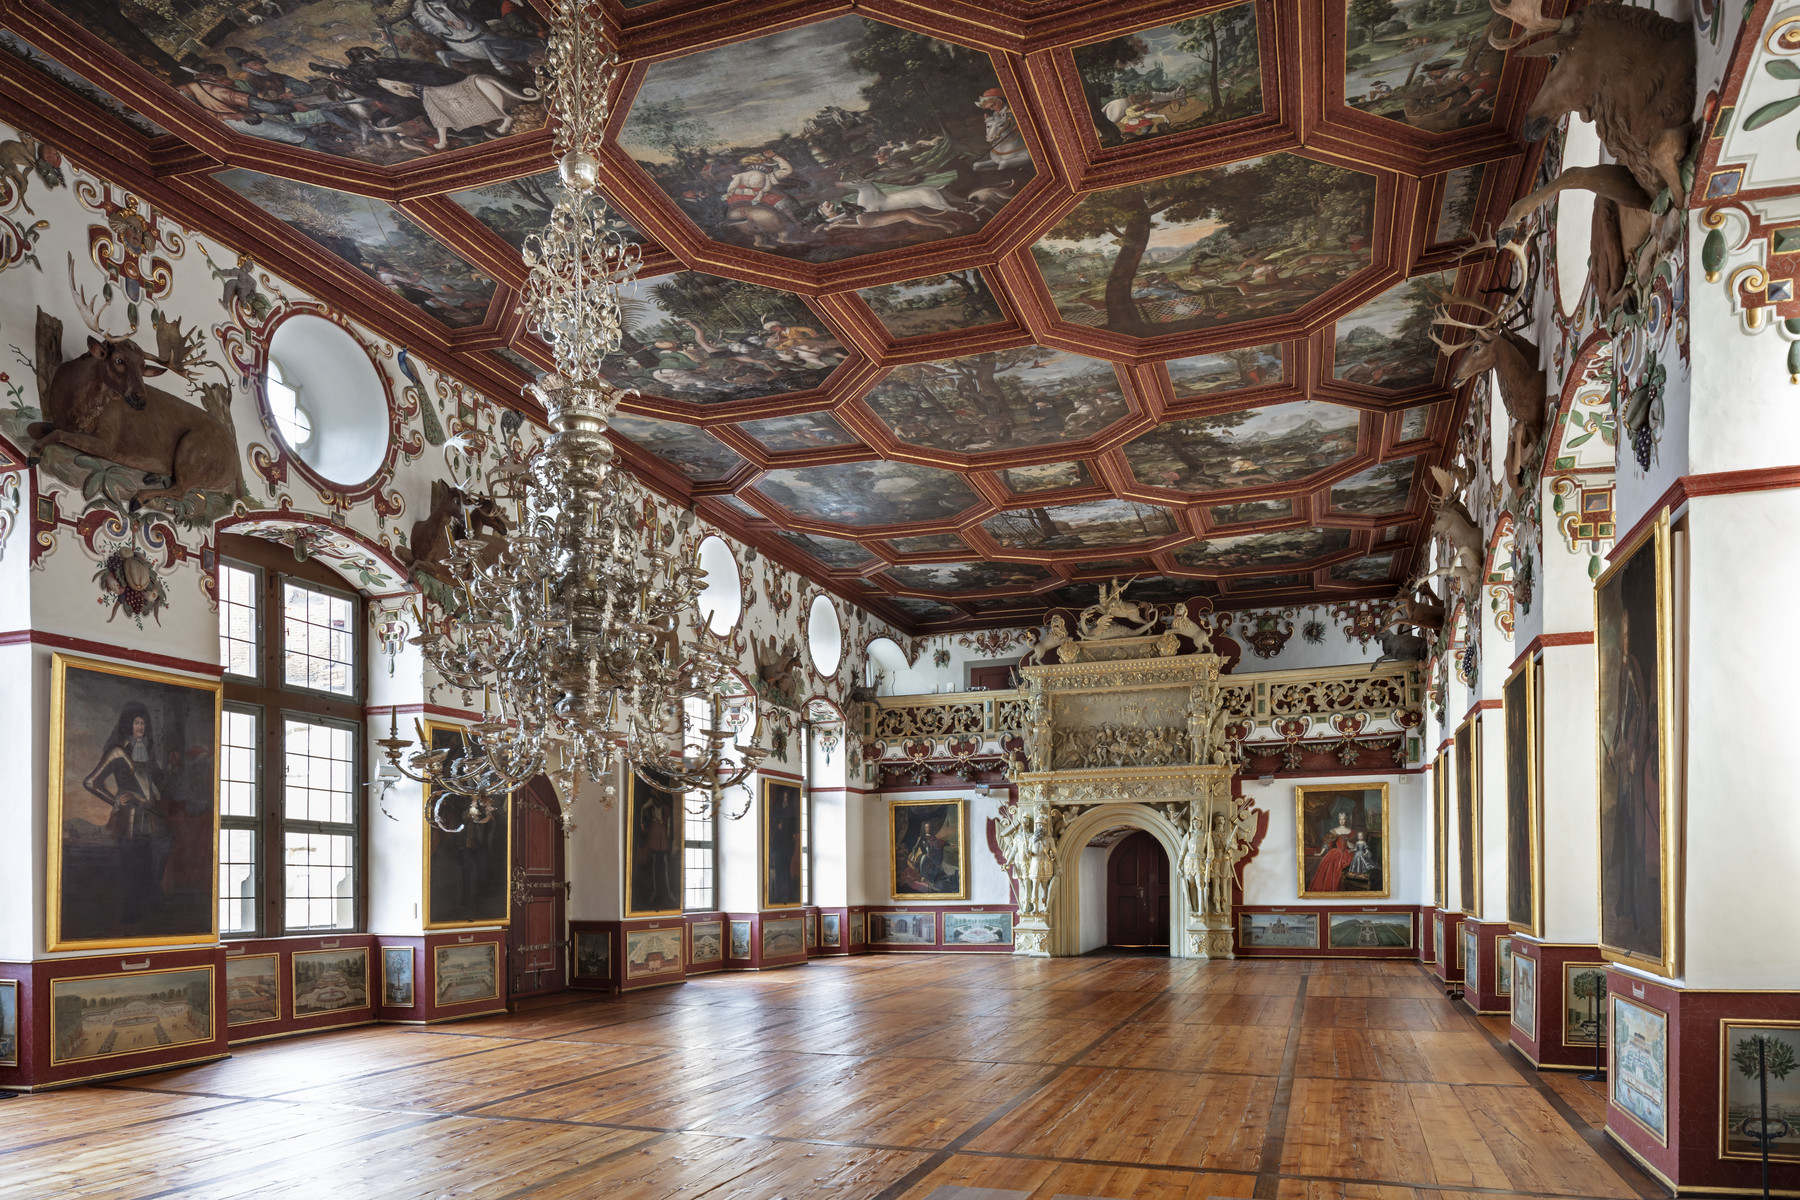
\includegraphics{impressum_files/mediabag/fmd10005862a.jpg}

}

\caption{Knight's Hall \& Room 72 - to the west}

\end{figure}%

Wikibase link:
\url{https://computational-publishing-service.wikibase.cloud/entity/Q213}

Title: Lion couple -- general view

Year: 2018

Description: Gerhardt Schmidt, sculptor - collaboration: Christoph
Limmerich, sculptor - collaboration: Caspar Dieterich, barrel painter -
Weikersheim, Weikersheim Castle, Knight's Hall \& Room 72 - Completion:
1605 - 1747

\begin{figure}[H]

{\centering 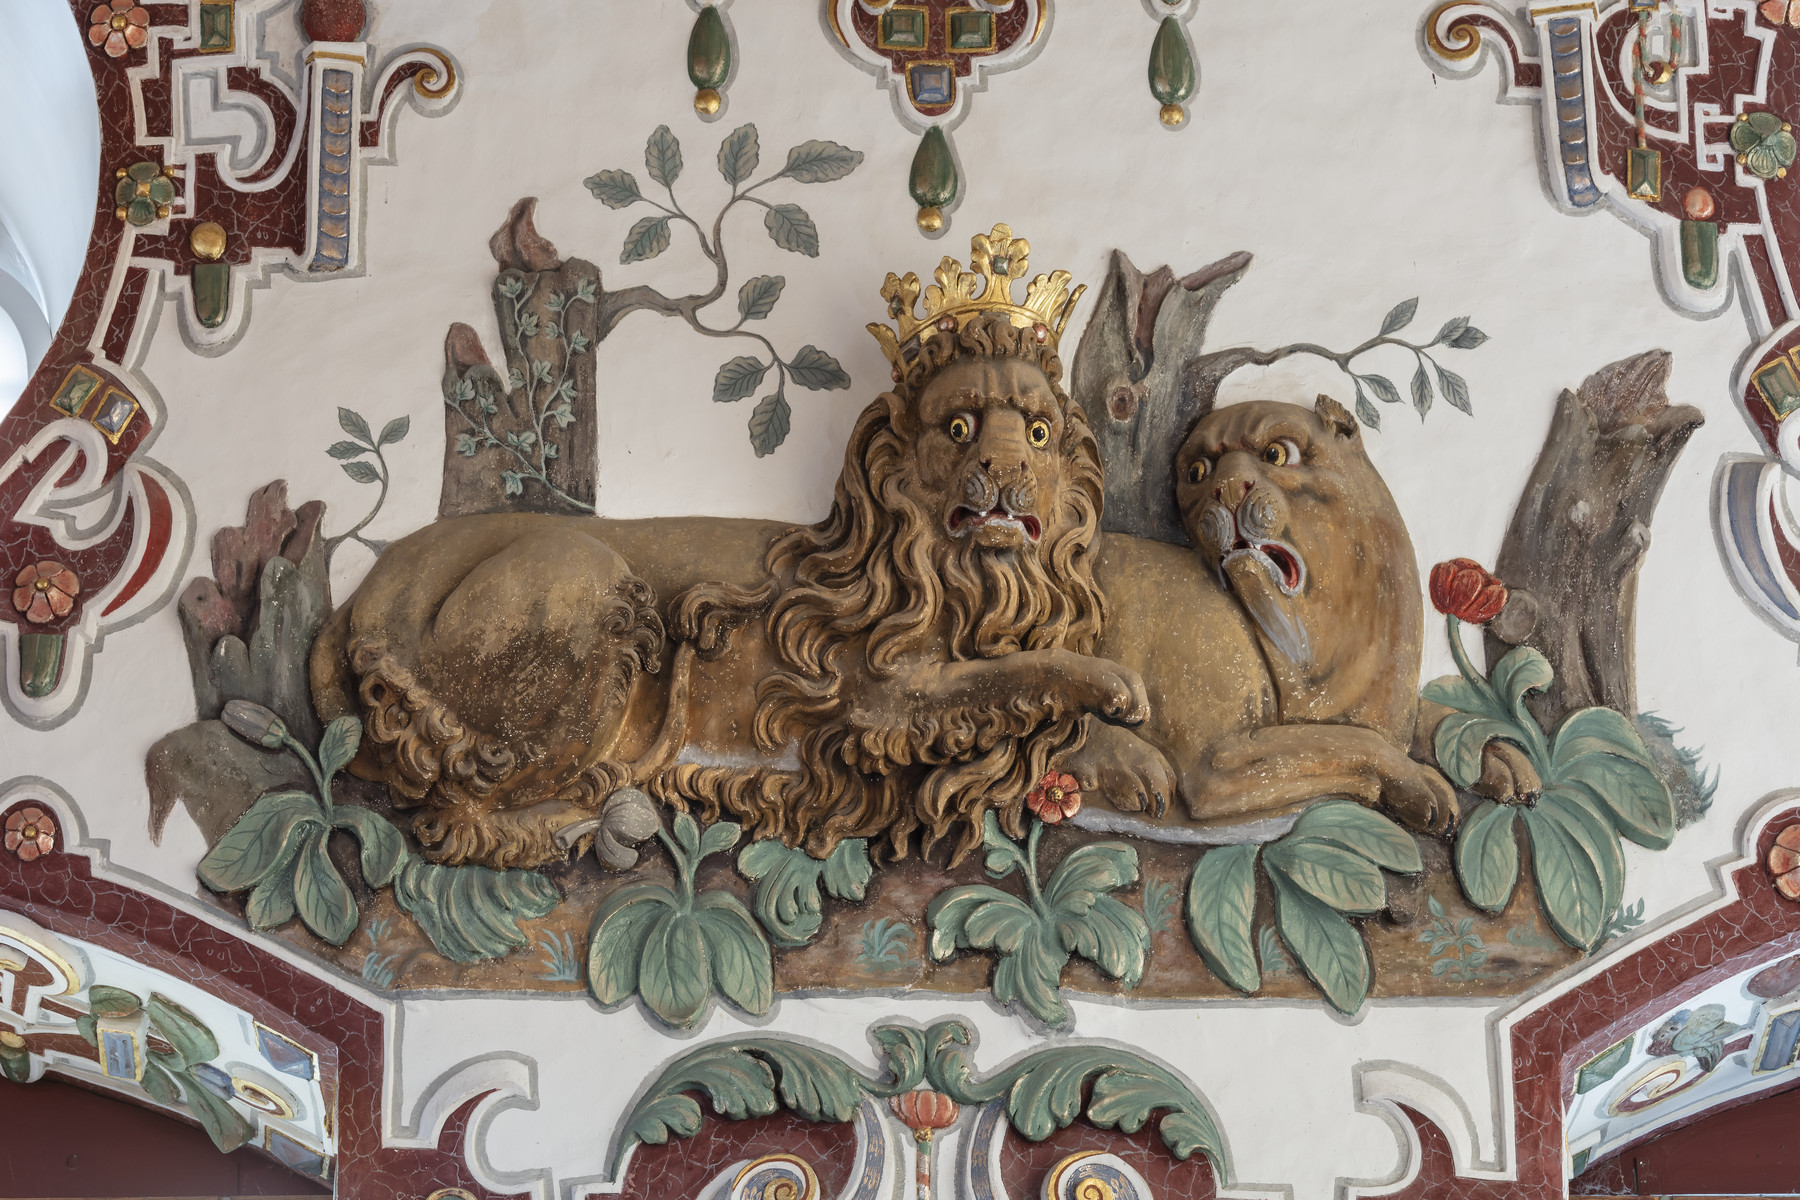
\includegraphics{impressum_files/mediabag/fmd10005864a.jpg}

}

\caption{Lion couple -- general view}

\end{figure}%

Wikibase link:
\url{https://computational-publishing-service.wikibase.cloud/entity/Q214}

Title: Bear -- general view

Year: 2018

Description: Gerhardt Schmidt, sculptor - collaboration: Christoph
Limmerich, sculptor - collaboration: Caspar Dieterich, barrel painter -
Weikersheim, Weikersheim Castle, Knight's Hall \& Room 72 - Completion:
1605 - 1747

\begin{figure}[H]

{\centering 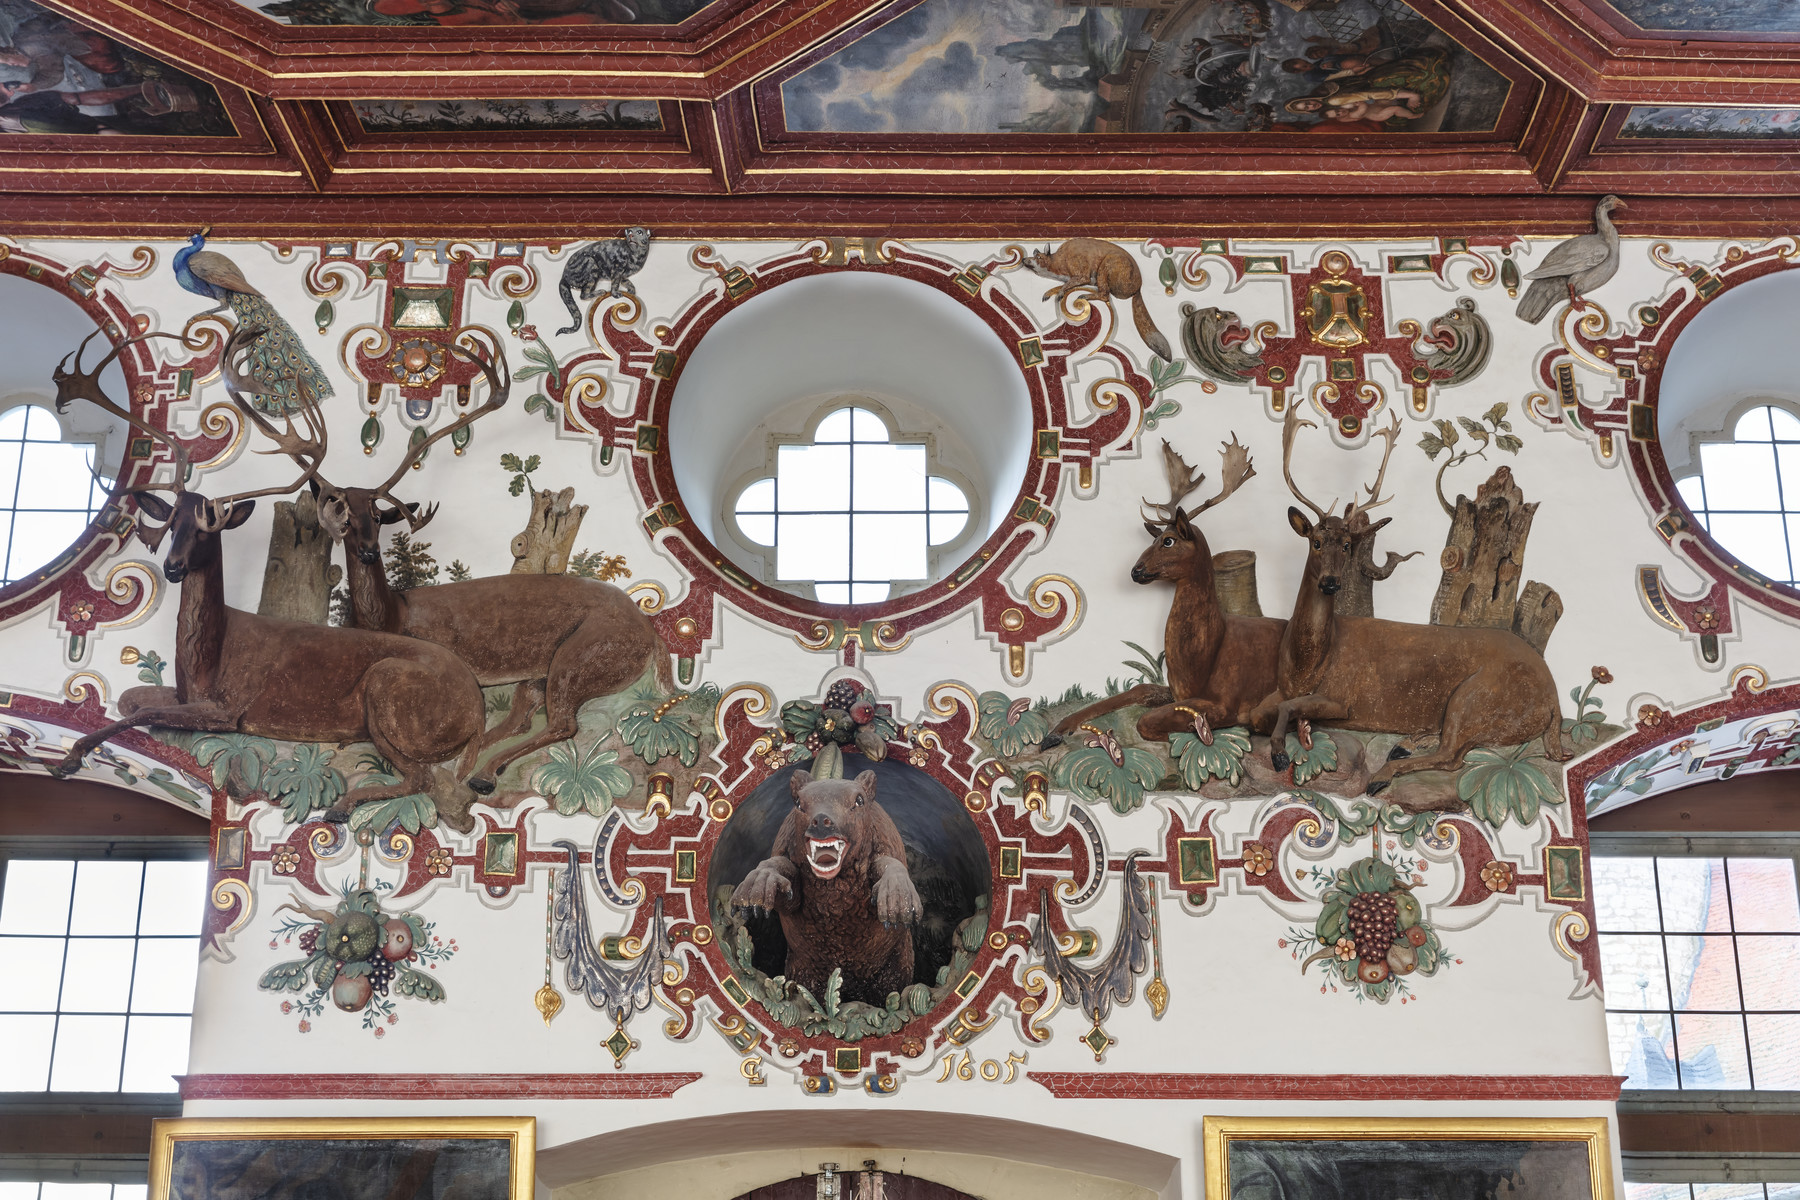
\includegraphics{impressum_files/mediabag/fmd10005865a.jpg}

}

\caption{Bear -- general view}

\end{figure}%

Wikibase link:
\url{https://computational-publishing-service.wikibase.cloud/entity/Q216}

Title: Monkey -- general view

Year: 2018

Description: Gerhardt Schmidt, sculptor - collaboration: Christoph
Limmerich, sculptor - collaboration: Caspar Dieterich, barrel painter -
Weikersheim, Weikersheim Castle, Knight's Hall \& Room 72 - Completion:
1605 - 1747

\begin{figure}[H]

{\centering 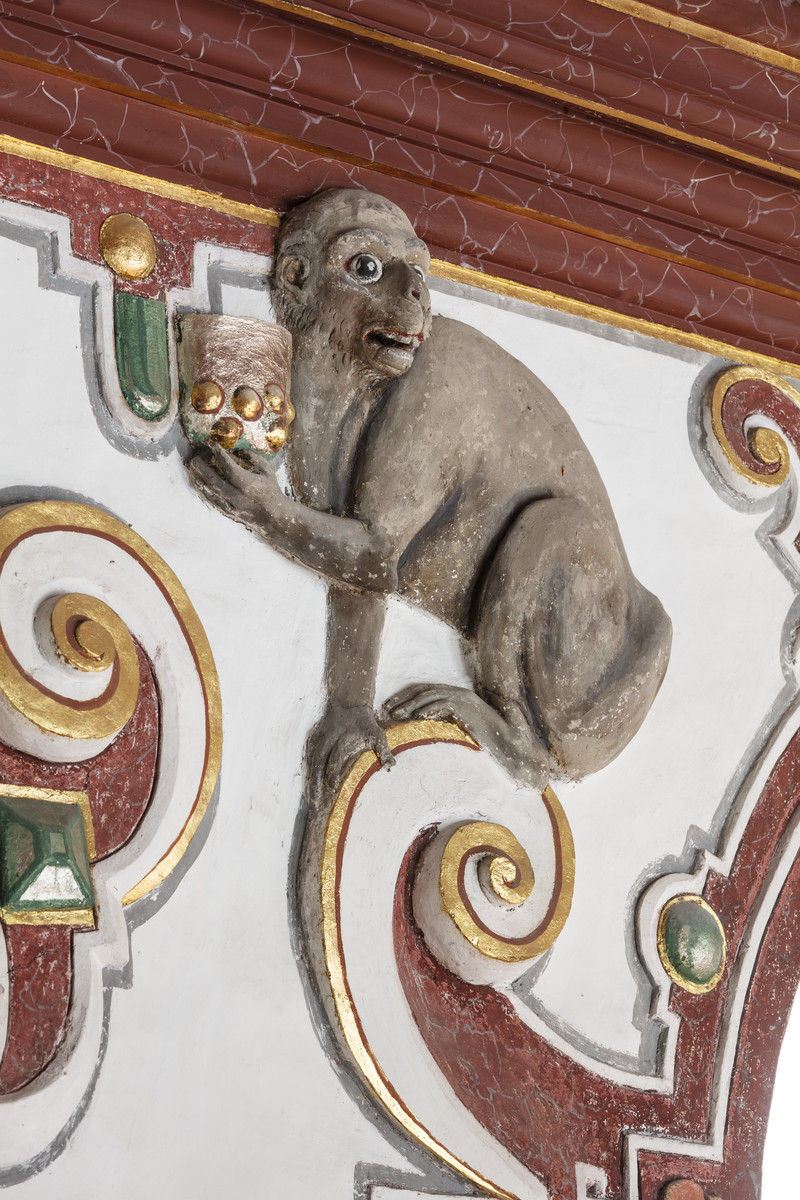
\includegraphics{impressum_files/mediabag/fmd10005867a.jpg}

}

\caption{Monkey -- general view}

\end{figure}%

Wikibase link:
\url{https://computational-publishing-service.wikibase.cloud/entity/Q215}

Title: Deer pairs -- general view

Year: 2018

Description: Gerhardt Schmidt, sculptor - collaboration: Christoph
Limmerich, sculptor - collaboration: Caspar Dieterich, barrel painter -
Weikersheim, Weikersheim Castle, Knight's Hall \& Room 72 - Completion:
1605 - 1747

\begin{figure}[H]

{\centering 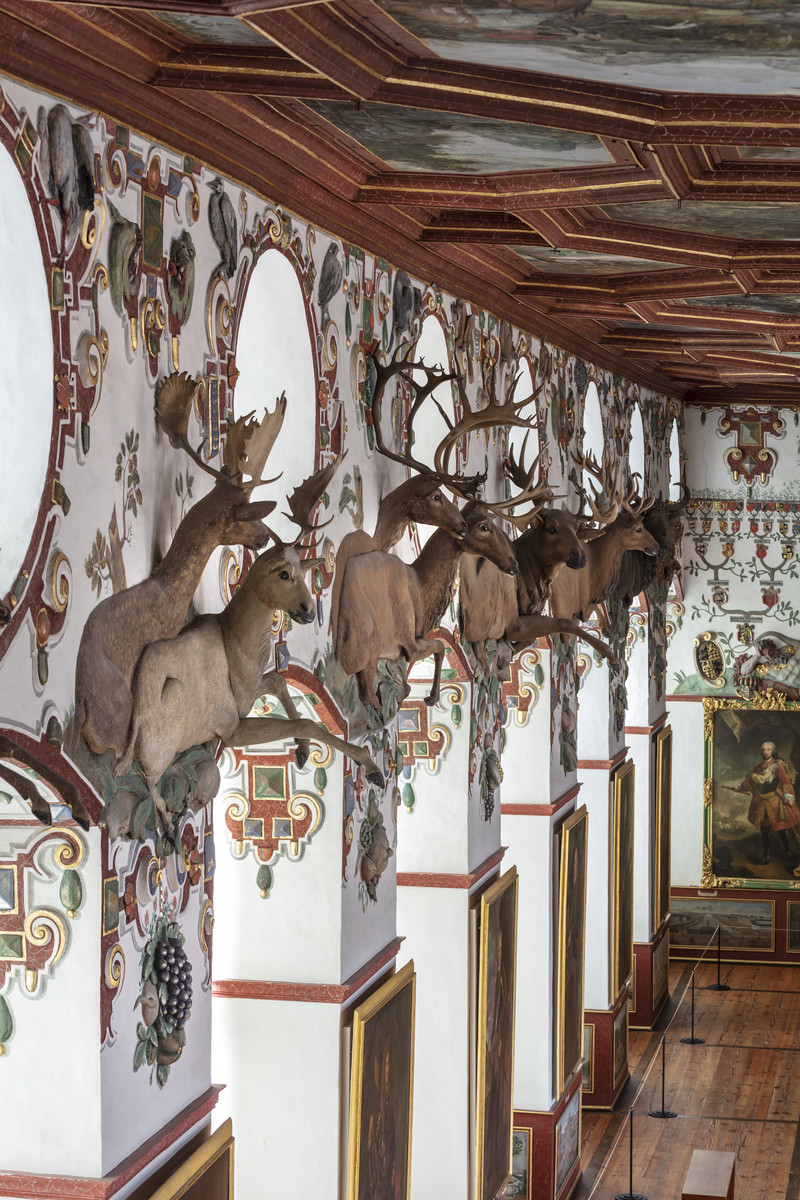
\includegraphics{impressum_files/mediabag/fmd10005866a.jpg}

}

\caption{Deer pairs -- general view}

\end{figure}%

Wikibase link:
\url{https://computational-publishing-service.wikibase.cloud/entity/Q200}

Title: Knight's Hall \& Room 72 - to the east

Year: 2018

Description: Part of: Weikersheim Castle SaalbauWolfgang Beringer,
builder \& Stonemason - Georg Stegle, master builder - design: Georges
Robin, architect - Elias Gunzenhäuser, carpenter - Weikersheim,
Marktplatz 11 - from 1595

\begin{figure}[H]

{\centering 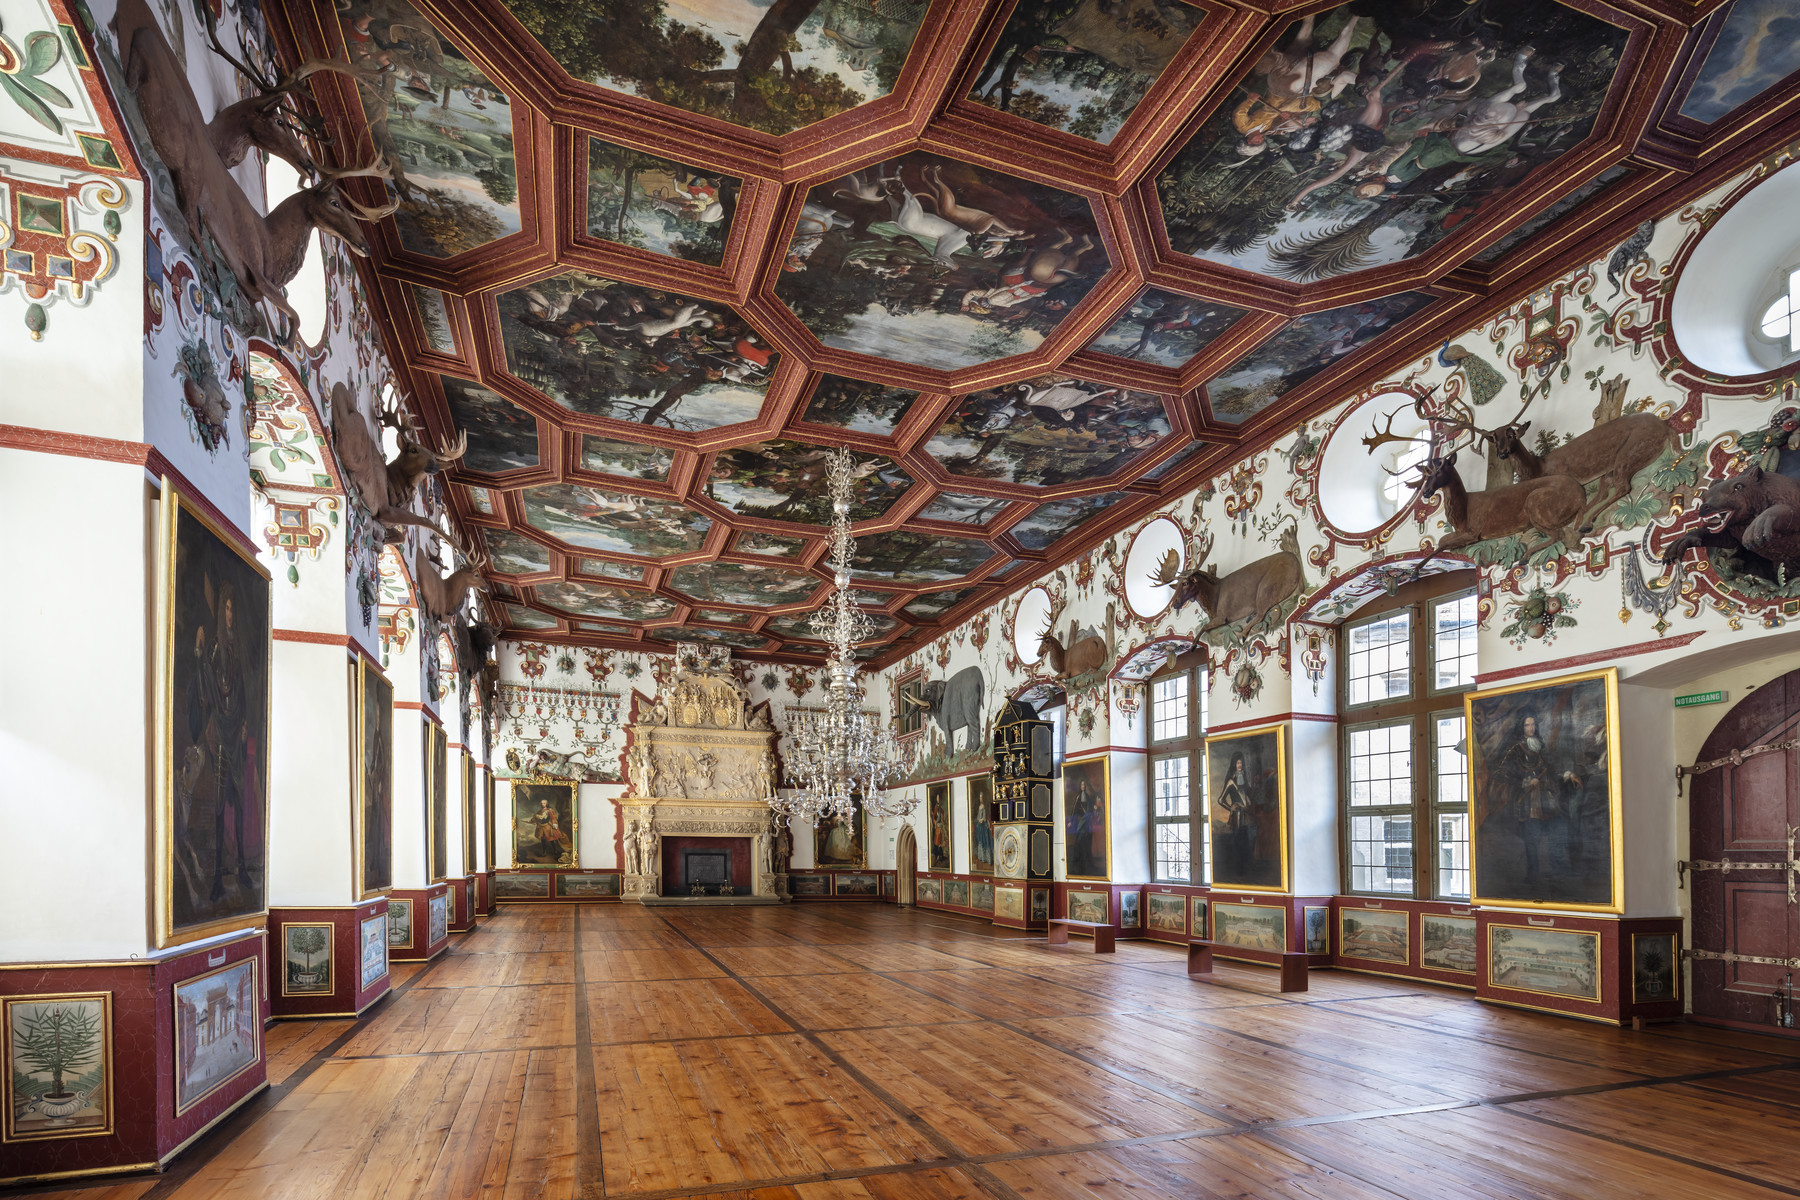
\includegraphics{impressum_files/mediabag/fmd10005859a.jpg}

}

\caption{Knight's Hall \& Room 72 - to the east}

\end{figure}%

Wikibase link:
\url{https://computational-publishing-service.wikibase.cloud/entity/Q211}

Title: Knight's Hall \& Room 72 - to the east

Year: 2018

Description: Part of: Weikersheim Castle Saalbau Wolfgang Beringer,
builder \& Stonemason - Georg Stegle, master builder - design: Georges
Robin, architect - Elias Gunzenhäuser, carpenter - Weikersheim,
Marktplatz 11 - from 1595

\begin{figure}[H]

{\centering 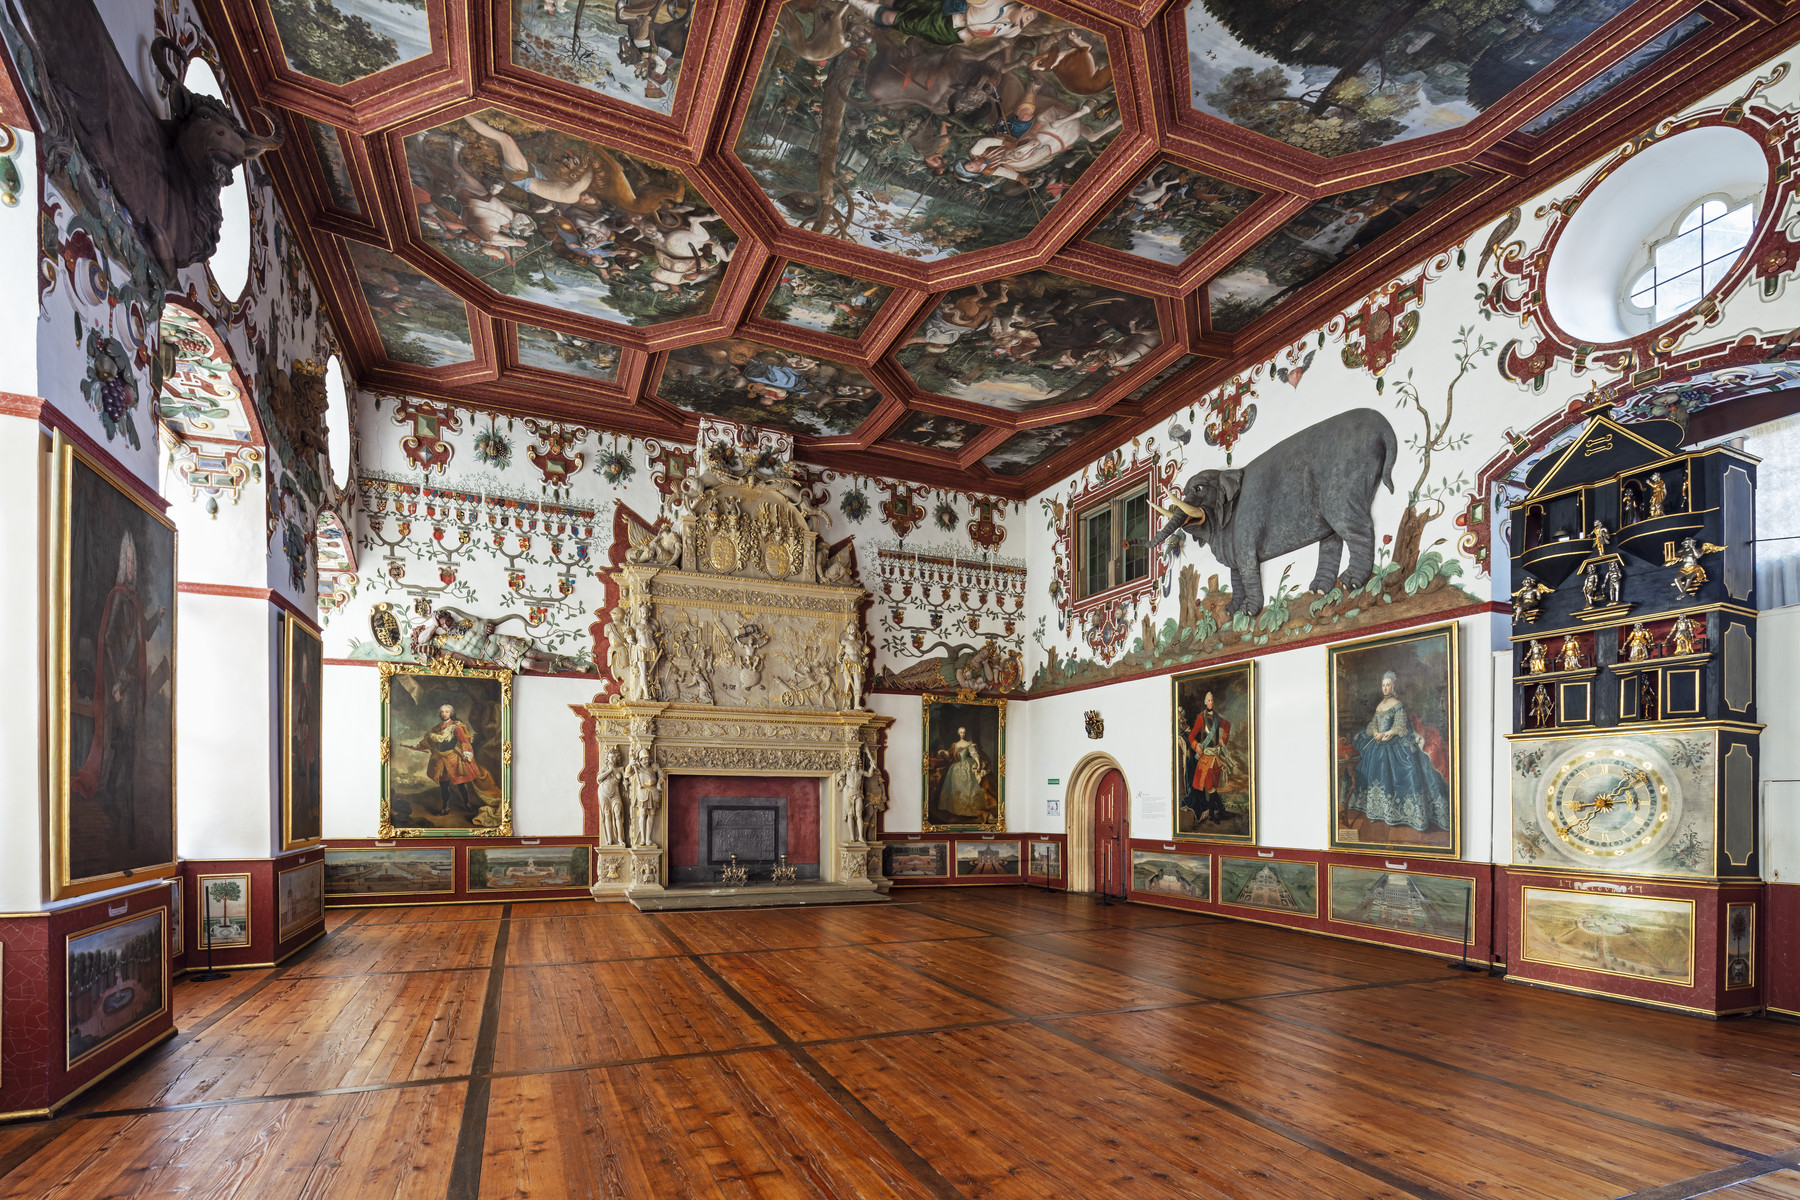
\includegraphics{impressum_files/mediabag/fmd10005860a.jpg}

}

\caption{Knight's Hall \& Room 72 - to the east}

\end{figure}%

\begin{verbatim}
C:\Users\worthingtons\AppData\Local\Packages\PythonSoftwareFoundation.Python.3.11_qbz5n2kfra8p0\LocalCache\local-packages\Python311\site-packages\VizKG\utils\util.py:89: UserWarning: Could not infer format, so each element will be parsed individually, falling back to `dateutil`. To ensure parsing is consistent and as-expected, please specify a format.
  dataframe[column] = dataframe[column].astype('datetime64')
C:\Users\worthingtons\AppData\Local\Packages\PythonSoftwareFoundation.Python.3.11_qbz5n2kfra8p0\LocalCache\local-packages\Python311\site-packages\VizKG\utils\util.py:89: UserWarning: Could not infer format, so each element will be parsed individually, falling back to `dateutil`. To ensure parsing is consistent and as-expected, please specify a format.
  dataframe[column] = dataframe[column].astype('datetime64')
\end{verbatim}

\includegraphics{rittersaal_files/figure-pdf/cell-5-output-2.png}

\bookmarksetup{startatroot}

\chapter{Gemälde-Sammlung: Wikidata
benchmark}\label{gemuxe4lde-sammlung-wikidata-benchmark}

Objective: Make a selection of nine paintings for the exhibition
catalogue to be selected from Wikidata and rendered multi-format in
Quarto.

The below Python code uses SPARQLWrapper to retrieve data from Wikidata
based on a SPARQL query.

This page acts as a `benchmark' to test if data fields can be read from
Wikidata.

Wikidata link: \url{http://www.wikidata.org/entity/Q29474642}

Title: The Birth of Benjamin

Year: 1650

Creator: Francesco Furini

Copyright: public domain

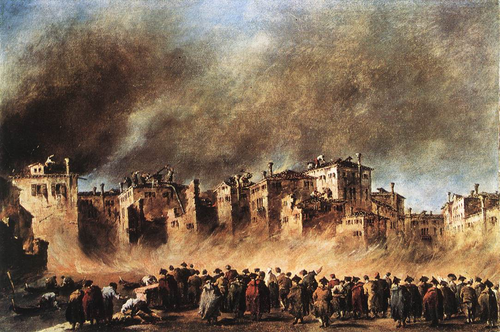
\includegraphics{painting-collection_files/figure-pdf/cell-2-output-2.png}

Wikidata link: \url{http://www.wikidata.org/entity/Q29474644}

Title: Venetian Gala Concert

Year: 1782

Creator: Francesco Guardi

Copyright: public domain

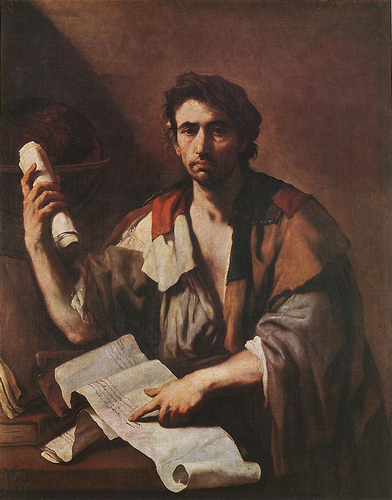
\includegraphics{painting-collection_files/figure-pdf/cell-2-output-4.png}

Wikidata link: \url{http://www.wikidata.org/entity/Q29474645}

Title: Q29474645

Year: 1789

Creator: Francesco Guardi

Copyright: public domain

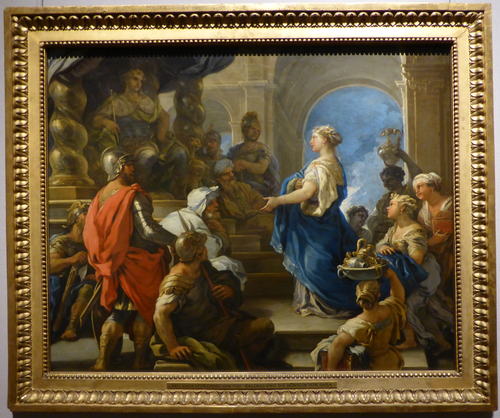
\includegraphics{painting-collection_files/figure-pdf/cell-2-output-6.png}


\backmatter


\end{document}
